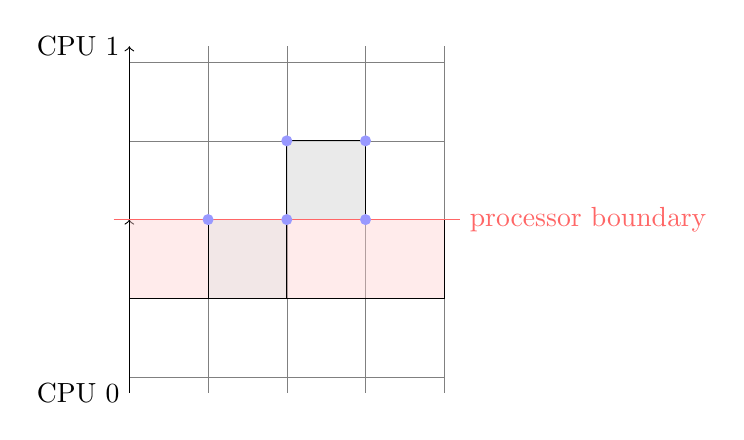
\begin{tikzpicture}[domain=-0.2:4.2]
    \draw[very thin,color=gray] (0,-0.2) grid (4,4.2);
    \draw[<-] (0,2) -- (0,-0.2) node[left] {CPU 0};
    \draw[->] (0,2) -- (0,4.2) node[left] {CPU 1};
    
    \filldraw[fill=gray!20,fill opacity=0.8](2,2)--(2,3)--(3,3)--(3,2)--cycle;
    \filldraw[fill=red!20,fill opacity=0.4](0,1)--(4,1)--(4,2)--(0,2)--cycle;
    \filldraw[fill=gray!20,fill opacity=0.5](1,1)--(2,1)--(2,2)--(1,2)--cycle;
    
    \draw[color=red!60,-] (-0.2,2) -- (4.2,2) node[right] {processor boundary};
    
    \fill[blue!40] (2,2) circle (2pt);
    \fill[blue!40] (2,3) circle (2pt);
    \fill[blue!40] (3,3) circle (2pt);
    \fill[blue!40] (3,2) circle (2pt);
    
    \fill[blue!40] (1,2) circle (2pt);

\end{tikzpicture}
